% vim: set spell spelllang=es syntax=tex :

\section{Descripción del framework}

Para aumentar el throughput del sistema se aplicaran las dos técnicas discutidas
con anterioridad. La primer optimización consta en dividir cada cuadro para que
cada parte pueda ser procesada por un hilo distinto. La segunda optimización
sera que el sistema no estará limitado a tomar solo un cuadro por ves. Para
controlar estas dos optimizaciones debemos definir dos parámetros. Para la
primera establecemos la cantidad de partes en las cuales se dividirá cada ítem,
mientras que para la segunda establecemos la cantidad máxima de tareas de
búsqueda en ejecución.

También seria deseable que las distintas pilas de plugins ejecuten de forma
independiente una de la otra para que el retardo de procesamiento de cada cuadro
sea menor. Sin embargo, en los experimentos realizados se comprobó que el
overhead y la competencia de recursos introducidos por el incremento en la
cantidad de tareas afecta de forma notable el rendimiento de la aplicación, por
lo cual se opto que las pilas ejecuten de forma secuencial.

Conceptualmente el framework ejecutara cuatro tipos de tareas distintos, que a
su ves pueden ser divididos en tareas persistentes y tareas de búsqueda. Las
primeras son aquellas de las cuales solo habrá una instancia y permanecerán
durante la ejecución la mayor parte del programa, mientra que definimos a las
tareas de búsqueda a aquellas creadas con el objetivo de procesar un único
cuadro (o un fragmento de uno), y que terminaran cuando terminen de procesar
este. Las tareas persistentes son generación de ítems y generación de tareas de
búsqueda, mientras que las tareas de búsqueda son fractura de ítems y
procesamiento de fragmentos.

\begin{description}

\item[Generación de ítems:] Sera la encargada de la generación o captura de los
	ítems y colocarlos en la cola de ítems a procesar. Solo habrá una
	instancia de esta tarea.

\item[Generación de tareas de búsqueda:] Esta tarea sera la encargada de tomar
	un ítem de la cola de ítems a procesar cuando la cantidad de tareas en
	ejecución sea menor que el máximo establecido, y crear una tarea de
	fractura para este. Solo habrá una instancia de esta tarea.

\item[Fractura de ítems:] Cada una de estas tareas dividirá el ítem en tantas
	partes como se haya definido al comienzo de la ejecución y por cada
	fragmento creara una tarea de procesamiento de fragmentos asociada a
	este.

\item[Procesamiento de fragmentos:] Cada una de estas tareas tomara su fragmento
	asociado y lo procesara utilizando cada una de las pilas de plugins.

\end{description}

TODO: Diagrama del framework

\section{Implementación del framework}

El framework fue implementado en \emph{C++} utilizando \emph{OpenMP}. La
elección del lenguaje principalmente se debe al deseo de trabajar tomando como
base el desarrollo realizado por Torres en \cite{torres2014}, en especial se
espero hacer uso de los plugins. Por su parte, el autor original del software
eligió este lenguaje debido a su eficiencia y paradigma. Dado que el sistema
debe procesar los cuadros en tiempos acotados, la eficiencia es es crucial,
mientras que el paradigma orientado a objetos permite establecer fácilmente la
interfaz de los plugins. Por otra parte, utilizar \emph{OpenMP} es una
desviación del software original.

\emph{OpenMP} es una API de bibliotecas y directivas al compilador para la
definición de paralelismo de alto nivel para sistemas de memoria compartida en
\emph{C}, \emph{C++} y \emph{Fortran}\cite{ompWeb}. La ventaja de \emph{OpenMP}
es que permite la creación de regiones paralelas, secciones criticas, tareas y
puntos de sincronización, simplemente marcando un bloque de código con unas
pocas directivas al compilador. \emph{OpenMP} ademas provee la facilidad de que
se puede establecer la cantidad de hilos que irán ejecutando las tareas, y que
el orden de la cola de espera es \emph{frist-come/first-served}. Aun así se
mantiene un control del numero de tareas para no crear mas de las que pueden ser
procesadas, y no retrasar al sistema con tareas viejas.

Las clases del framework básico son las siguientes:

\begin{description}

\item[Item:] Esta clase define un tipo genérico de los ítems que serán tratados
	por el sistema.

\item[RingBuffer:] Este es el buffer donde se guardan los ítems generados
	mientras esperan ser procesados. El buffer guarda solo punteros a
	objetos de la clase \emph{Item} y no tiene mecanismos de control que
	permitan acceder la estructura desde múltiples threads al mismo tiempo
	de forma segura. Cuando se solicita un ítem, se devuelve el puntero al
	mas antiguo o \textbf{NULL} en caso de que la estructura este vacía.
	Cuando se intenta agregar un nuevo ítem pero la estructura esta llena se
	coloca este en espacio del ítem mas viejo en la estructura y se retorna
	el puntero de este al llamador, delegándole su destrucción.  La
	destrucción del ítem se delega al llamador por dos motivos. El primero
	es que el buffer desconoce el tipo real del ítem. La segunda razón es
	que para poder ser utilizado de forma segura, las llamadas a los métodos
	del buffer deben estar dentro de secciones criticas y realizar las
	eliminaciones dentro de estas podría ser muy lento. Si el dominio así lo
	requiere, se puede cambiar el comportamiento de esta clase para que
	funcione como una pila en lugar de una cola.

\item[Input:] Se trata de una clase que funciona como definición de la interfaz
	de las clases que generan los ítems. Sus métodos principales son
	\emph{run} y \emph{generate}. El método \emph{generate} debe ser re
	implementado por las clases hijas para generar el tipo de ítem
	especifico del sistema. El método \emph{run} es el encargado de generar
	los ítems llamando a \emph{generate} y colocarlos en el
	\emph{RingBuffer}. Este último método puede ser redefinido si la
	aplicación así lo requiere.

\item[ItemSlicer:] Es la clase que define la interfaz de las clases encargadas
	de dividir los ítems. Se definen tres métodos. El primero es
	\emph{slice} que recibe como parámetro ítem y la cantidad de partes en
	la que este debe ser dividido y retorna un arreglo de ítems. El segundo
	método es \emph{resetItem} que recibe como parámetro una de las partes
	creadas por el método \emph{slice} luego de que fue procesada por una
	pila de plugins y la configura al estado para que el funcionamiento de
	la próxima pila no se vea interferido. El tercer método es
	\emph{delPart} que recibe como parámetro un fragmento de ítem y lo
	elimina.

\item[Plugin:] Esta clase define una interfaz para los plugins que realizaran
	las distintas partes del procesamiento de la imagen. Solo se define el
	método \emph{process} que tiene como único parámetro un puntero a un
	objeto de la clase \emph{Item}.

\item[PluginStack:] Esta es la clase que tomara el ítem y se encarga de
	entregarlo a cada uno de los plugins. Tiene solo dos métodos,
	\emph{addPlugin}, para agregar un plugin, y \emph{process} que tiene
	como parámetro un ítem, para procesarlo.

\item[ItemSwitch:] Esta es la clase mas compleja del framework básico, ya que es
	la que crea las múltiples tareas. La primera tarea que crea es la
	encargada de consumir los ítems del buffer y crear las tareas de
	búsqueda. Cada tarea de búsqueda divide el ítem utilizando el
	\emph{ItemSlicer} y crea una nueva tarea por cada fragmento. Por último,
	las tarea de fragmento procesara cada fragmento con todas las pilas de
	plugins de forma secuencial.

\end{description}

\begin{figure}[h]

	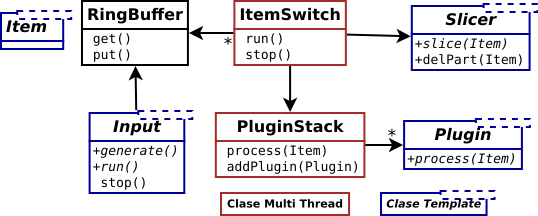
\includegraphics[width=\textwidth]{img/clasesFramework.pdf}

	\caption{Diagrama de clases Framework base.}

\end{figure}

Existen dos parámetros ajustables. El primero es la cantidad de hilos que
ejecutaran las tareas de búsqueda. El segundo parámetro es la cantidad de partes
en las cuales se dividirá el cuadro.

Para adaptar el framework para utilizarlo como un sistema de visión por
computadora para el fútbol de robots se incorporaron las siguientes clases, las
cuales fueron tomadas y modificadas del sistema de visión presentado en
\cite{torres2014}:

\begin{description}

\item[Frame:] Subclase de \emph{Item}. Contiene una imagen que representa un
	cuadro y una estructura auxiliar que contiene la información necesaria
	para el funcionamiento de los plugins.

\item[CaptureFromFile:] Subclase de \emph{Input}. Es la clase encargada de crear
	el flujo de objetos \emph{Frame}, tomando cada cuadro desde un archivo
	de vídeo. También debe respetar la taza de cuadros por segundo del
	vídeo.

\item[FastCaptureFromFile:] Subclase de \emph{Input}. Muy similar a
	\emph{CaptureFromFile}, con las diferencias de que carga los cuadros a
	memoria antes de que comience el sistema a capturar los cuadros (para
	evitar los retardos de la lectura de disco y decodificación), y si la
	cola de cuadros a procesar esta vacía, adelantara la creación del
	próximo cuadro. Esta clase es útil para comprobar la capacidad máxima
	del sistema.

\item[FrameSlicer:] Subclase de \emph{ItemSlicer}. En este caso lo que se divide
	es la imagen del cuadro. Cada sub cuadro tendrá un solapamiento con los
	adyacente ya que se debe evitar que un robots o la pelota no este
	totalmente contenido dentro de por lo menos un sub cuadro. Para
	minimizar el área solapada, las particiones se realizan de manera tal
	que se minimice el perímetro pero ocupen la mayor área posible. Para
	lograr esto se busca la partición que haga que la relación entre el alto
	y el ancho sea lo mas cercana a uno.

\item[Subclases de \emph{Plugin}:] \emph{PluginBlur},
	\emph{PluginColorConversions}, \emph{PluginColorSegmentation},
	\emph{PluginDetectBalls}, \emph{PluginFindBlobs},
	\emph{PluginFindSecondariesBlobs}, \emph{PluginMorphology} y
	\emph{PluginNetworking}.

\item[Clases auxiliares:] \emph{ball}, \emph{colorspace}, \emph{datastruct},
	\emph{homography}, \emph{marker}, \emph{pattern},
	\emph{pattern\_matching}, \emph{practicalsocket}, \emph{segmentation},
	\emph{team}, \emph{timer}.

\end{description}

\begin{figure}[h]

	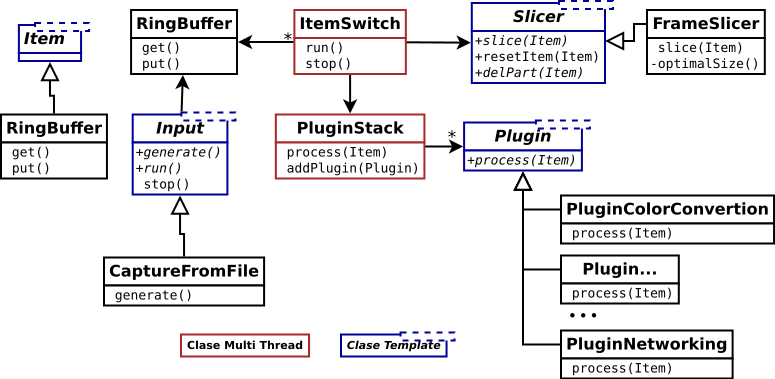
\includegraphics[width=\textwidth]{img/clasesFrameworkRobots.pdf}

	\caption{Diagrama de clases Framework del framework instanciado para el
	sistema de visión para el fútbol de robots.}

\end{figure}

Conceptualmente, la implementación para fútbol de robots tiene dos pilas, una
para búsqueda de robots y la otra para búsqueda de la pelota. Sin embargo, ambas
pilas para la etapa de pre procesamiento de la imagen utilizan los mismos
plugins con la misma configuración, ademas, los plugins que no tienen en común
solo modifican datos propios de cada pila. Esto permite que ambas pilas puedan
ser unidas en una sola, lo que trae como ventaja que la etapa de pre
procesamiento se realice solo una ves por cuadro.
